\documentclass[a4paper, 11pt]{article}

\usepackage[french]{babel}
\usepackage[utf8]{inputenc}
\usepackage[T1]{fontenc}
\usepackage{placeins}
\usepackage{csquotes}
\usepackage{hyperref}
\usepackage{amsmath}
\usepackage{tikz}
\usetikzlibrary{automata,arrows,positioning}
\usepackage{graphicx}

\graphicspath{{img/}}

\author{Florian Thuin \and Cyril de Vogelaere}
\date{\today}
\title{Assignment 2: Deeper understanding of j-- compiler}

\begin{document}
    \maketitle
    \tableofcontents
    \section{Lexical analysis}
    Here is a regExp:
    $$ ((a^{*}b) \mid {(ab)}^{*})c $$

    With this regExp, we can define an infinite number of sequences:

    $$ \{ \epsilon, c, bc, abc, aabc, ababc, \ldots \} $$

    \subsection{NFA with Thompson construction}

    \begin{figure}[!ht]
    	\begin{center}
    		\begin{tikzpicture}[node distance=2cm, on grid, auto]
                \node[state, initial, initial text={}] (0) {$0$};
                \node[state, above right =of 0] (1)  {$1$};
                \node[state, below right =of 0] (2)  {$2$};
                \node[state, above right =of 1] (3)  {$3$};
                \node[state, right of = 3]      (4)  {$4$};
                \node[state, below right =of 4] (5)  {$5$};
                \node[state, right of = 5]      (6)  {$6$};
                \node[state, below right =of 6] (7)  {$7$};
                \node[state, below right =of 2] (8)  {$8$};
                \node[state, right of = 8] (9)  {$9$};
                \node[state, right of = 9] (10) {$10$};
                \node[state, above right =of 10] (11) {$11$};
                \node[state, accepting, right of = 7] (12) {$12$};

                \path[->, line width=2pt] (0) edge node {$\epsilon$} (1);
                \path[->, line width=2pt] (0) edge node {$\epsilon$} (2);
                \path[->, line width=2pt] (1) edge node {$\epsilon$} (3);
                \path[->, line width=2pt] (4) edge node {$\epsilon$} (5);
                \path[->, line width=2pt] (5) edge node {$b$} (6);
                \path[->, line width=2pt] (1) edge node {$\epsilon$} (5);
                \path[->, line width=2pt] (6) edge node {$\epsilon$} (7);
                \path[->, line width=2pt] (2) edge node {$\epsilon$} (11);
                \path[->, line width=2pt] (2) edge node {$\epsilon$} (8);
                \path[->, line width=2pt] (9) edge node {$b$} (10);
                \path[->, line width=2pt] (11) edge node {$\epsilon$} (7);
                \path[->, line width=2pt] (7) edge node {$c$} (12);
                \path[->, line width=2pt] (10) edge node {$\epsilon$} (11);
                \path[->, line width=2pt] (8) edge node {$a$} (9);
                \path[->, line width=2pt] (3) edge [bend left] node {$a$} (4);
                \path[->, line width=2pt] (4) edge [bend left] node {$\epsilon$} (3);
                \path[->, line width=2pt] (10) edge [bend left] node {$\epsilon$} (8);
            \end{tikzpicture}
    	\caption{NFA of $(({a}^{*}b)|{(ab)}^{*})c$}
    	\end{center}
    \end{figure}

    \subsection{NFA to DFA step-by-step}

    First we regroup all the states reachable from the initial only by using
    $\epsilon$-closure (i.e.\ reachable only with $\epsilon$-transitions).

    \begin{figure}[!ht]
        \begin{center}
        \begin{tikzpicture}
            \node[state, initial, initial text={}] (0) {$0,1,2,3,5,7,8,11$};
        \end{tikzpicture}
        \caption{NFA to DFA\@: Initial state}
        \end{center}
    \end{figure}

    Then, we add which states are reachable from this initial state with an
    $a$-transition (including $\epsilon$-transition):

    \begin{figure}[!ht]
        \begin{center}
        \begin{tikzpicture}[node distance=3cm, on grid, auto]
            \node[state, initial, initial text={}] (0) {$0,1,2,3,5,7,8,11$};
            \node[state, right of = 0] (1) {$4,5,9$};
            \path[->, line width=2pt] (0) edge node {$a$} (1);
        \end{tikzpicture}
        \caption{NFA to DFA\@: Initial state and an $a$-transition}
        \end{center}
    \end{figure}

    Then, we add which states are reachable from those states with a
    $b$-transition:

    \begin{figure}[!ht]
        \begin{center}
        \begin{tikzpicture}[node distance=3cm, on grid, auto]
            \node[state, initial, initial text={}] (0) {$0,1,2,3,5,7,8,11$};
            \node[state, right of = 0] (1) {$3,4,5,9$};
            \node[state, below of = 0] (2) {$6,7$};
            \node[state, below of = 1] (3) {$6,7,8,10,11$};
            \path[->, line width=2pt] (0) edge node {$a$} (1);
            \path[->, line width=2pt] (0) edge node {$b$} (2);
            \path[->, line width=2pt] (1) edge node {$b$} (3);
        \end{tikzpicture}
        \caption{NFA to DFA\@: Initial state and an $a$-transition and a $b$-transition}
        \end{center}
    \end{figure}

    Then, we add which states are reachable from those states with an $a$-transition:
    \begin{figure}[!ht]
        \begin{center}
        \begin{tikzpicture}[node distance=3cm, on grid, auto]
            \node[state, initial, initial text={}] (0) {$0,1,2,3,5,7,8,11$};
            \node[state, right of = 0] (1) {$3,4,5,9$};
            \node[state, below of = 0] (2) {$6,7$};
            \node[state, below of = 1] (3) {$6,7,8,10,11$};
            \node[state, right of = 1] (4) {$3,4,5$};
            \node[state, right of = 3] (5) {$9$};
            \path[->, line width=2pt] (0) edge node {$a$} (1);
            \path[->, line width=2pt] (0) edge node {$b$} (2);
            \path[->, line width=2pt] (1) edge node {$b$} (3);
            \path[->, line width=2pt] (1) edge node {$a$} (4);
            \path[->, line width=2pt] (3) edge node {$a$} (5);
        \end{tikzpicture}
        \caption{NFA to DFA\@: Initial state and two $a$-transitions and a $b$-transition}
        \end{center}
    \end{figure}

    We skip some steps by adding the remaining $a$- and $b$-transitions.

    \begin{figure}[!ht]
        \begin{center}
        \begin{tikzpicture}[node distance=3cm, on grid, auto]
            \node[state, initial, initial text={}] (0) {$0,1,2,3,5,7,8,11$};
            \node[state, right of = 0] (1) {$3,4,5,9$};
            \node[state, below of = 0] (2) {$6,7$};
            \node[state, right of = 1] (3) {$6,7,8,10,11$};
            \node[state, below of = 1] (4) {$3,4,5$};
            \node[state, right of = 3] (5) {$9$};
            \node[state, below of = 5] (7) {$7,8,10,11$};
            \path[->, line width=2pt] (0) edge node {$a$} (1);
            \path[->, line width=2pt] (0) edge node {$b$} (2);
            \path[->, line width=2pt] (1) edge node {$b$} (3);
            \path[->, line width=2pt] (1) edge node {$a$} (4);
            \path[->, line width=2pt] (3) edge [bend left] node {$a$} (5);
            \path[->, line width=2pt] (4) edge [loop below] node {$a$} (4);
            \path[->, line width=2pt] (4) edge node {$b$} (2);
            \path[->, line width=2pt] (5) edge [bend left] node {$b$} (7);
            \path[->, line width=2pt] (7) edge [bend left] node {$a$}(5);
        \end{tikzpicture}
        \caption{NFA to DFA\@: Initial state and two $a$-transitions and a $b$-transition}
        \end{center}
    \end{figure}

    We add the $c$-transitions:

    \begin{figure}[!ht]
        \begin{center}
        \begin{tikzpicture}[node distance=3cm, on grid, auto]
            \node[state, initial, initial text={}] (0) {$0,1,2,3,5,7,8,11$};
            \node[state, right of = 0] (1) {$3,4,5,9$};
            \node[state, below of = 0] (2) {$6,7$};
            \node[state, right of = 1] (3) {$6,7,8,10,11$};
            \node[state, below of = 1] (4) {$3,4,5$};
            \node[state, right of = 3] (5) {$9$};
            \node[accepting, state, below of = 2] (6) {$12$};
            \node[state, below of = 5] (7) {$7,8,10,11$};
            \path[->, line width=2pt] (5) edge [bend left] node {$b$} (7);
            \path[->, line width=2pt] (7) edge [bend left] node {$a$}(5);
            \path[->, line width=2pt] (0) edge node {$a$} (1);
            \path[->, line width=2pt] (0) edge node {$b$} (2);
            \path[->, line width=2pt] (1) edge node {$b$} (3);
            \path[->, line width=2pt] (1) edge node {$a$} (4);
            \path[->, line width=2pt] (3) edge [bend left] node {$a$} (5);
            \path[->, line width=2pt] (4) edge [loop below] node {$a$} (4);
            %\path[->, line width=2pt] (5) edge [bend left] node {$b$} (3);
            \path[->, line width=2pt] (4) edge node {$b$} (2);
            \path[->, line width=2pt] (0) edge [bend right] node {$c$} (6);
            \path[->, line width=2pt] (2) edge node {$c$} (6);
            \path[->, line width=2pt] (3) edge [bend left=45] node {$c$} (6);
            \path[->, line width=2pt] (7) edge [bend left] node {$c$} (6);
        \end{tikzpicture}
        \caption{NFA to DFA\@: Initial state and two $a$-transitions and a $b$-transition}
        \end{center}
    \end{figure}


    \section{Parsing}
    \section{DFA}
    	Yes, it is possible to accept an infinite language, for example
    	((1)* 0) accept an infinite sequence of bit but can be
    	represented by the following DFA :

    	\begin{figure}[!h]
    		\center
    		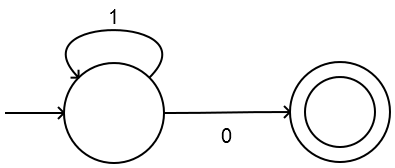
\includegraphics[scale=0.5]{DFAQ3.png}
    	\end{figure}

    \section{Language}
    	The language of balanced parenthesis is not regular.
    	To demonstrate it, let us consider a simplified version of the language
    	where we consider only a sequence of k left parenthesis followed by
    	a sequence of k right parenthesis, this simplified version forming
    	a subset of the language we wish to prove irregular :
    	\newline
    	$$\{(^k )^k\}$$

    	Using pumping lemmas, we can easily prove this language irregular by defining
    	$w = \{(^k )^k\}$. By the pumping lemma, there should be some decomposition
    	w = xyz with $|xy| \le p$ and $|y| \ge 1$ such that $x(y^i)z$
    	in L for every $i \ge 0$. \newline

    	Since $|xy| \le p$, we know that y can only contain a non-null sequence of
    	left parenthesis. This means that by pumping y and obtaining $xy^2 z$, we will
    	a sequence of parenthesis with more open parenthesis than closed parenthesis.
    	\newline

    	Thus, this sequence will never be part of our simplified language L, and since
    	this subset of the original language cannot be represent by a regular expression,
    	we can infer that the whole language similarly cannot be represented.

\end{document}
